\documentclass{article}

\usepackage{graphicx}
\usepackage{tikz}
\usepackage{tikzsymbols}
\usetikzlibrary{calc,patterns,shapes.geometric}
\pagestyle{empty}
\usepackage[margin=0pt]{geometry}
\geometry{papersize={14in,12in}}

\def\centerarc[#1](#2)(#3:#4:#5){\draw[#1] ($(#2)+({#5*cos(#3)},{#5*sin(#3)})$) arc (#3:#4:#5);}

\begin{document}
	\begin{figure}
		\centering
		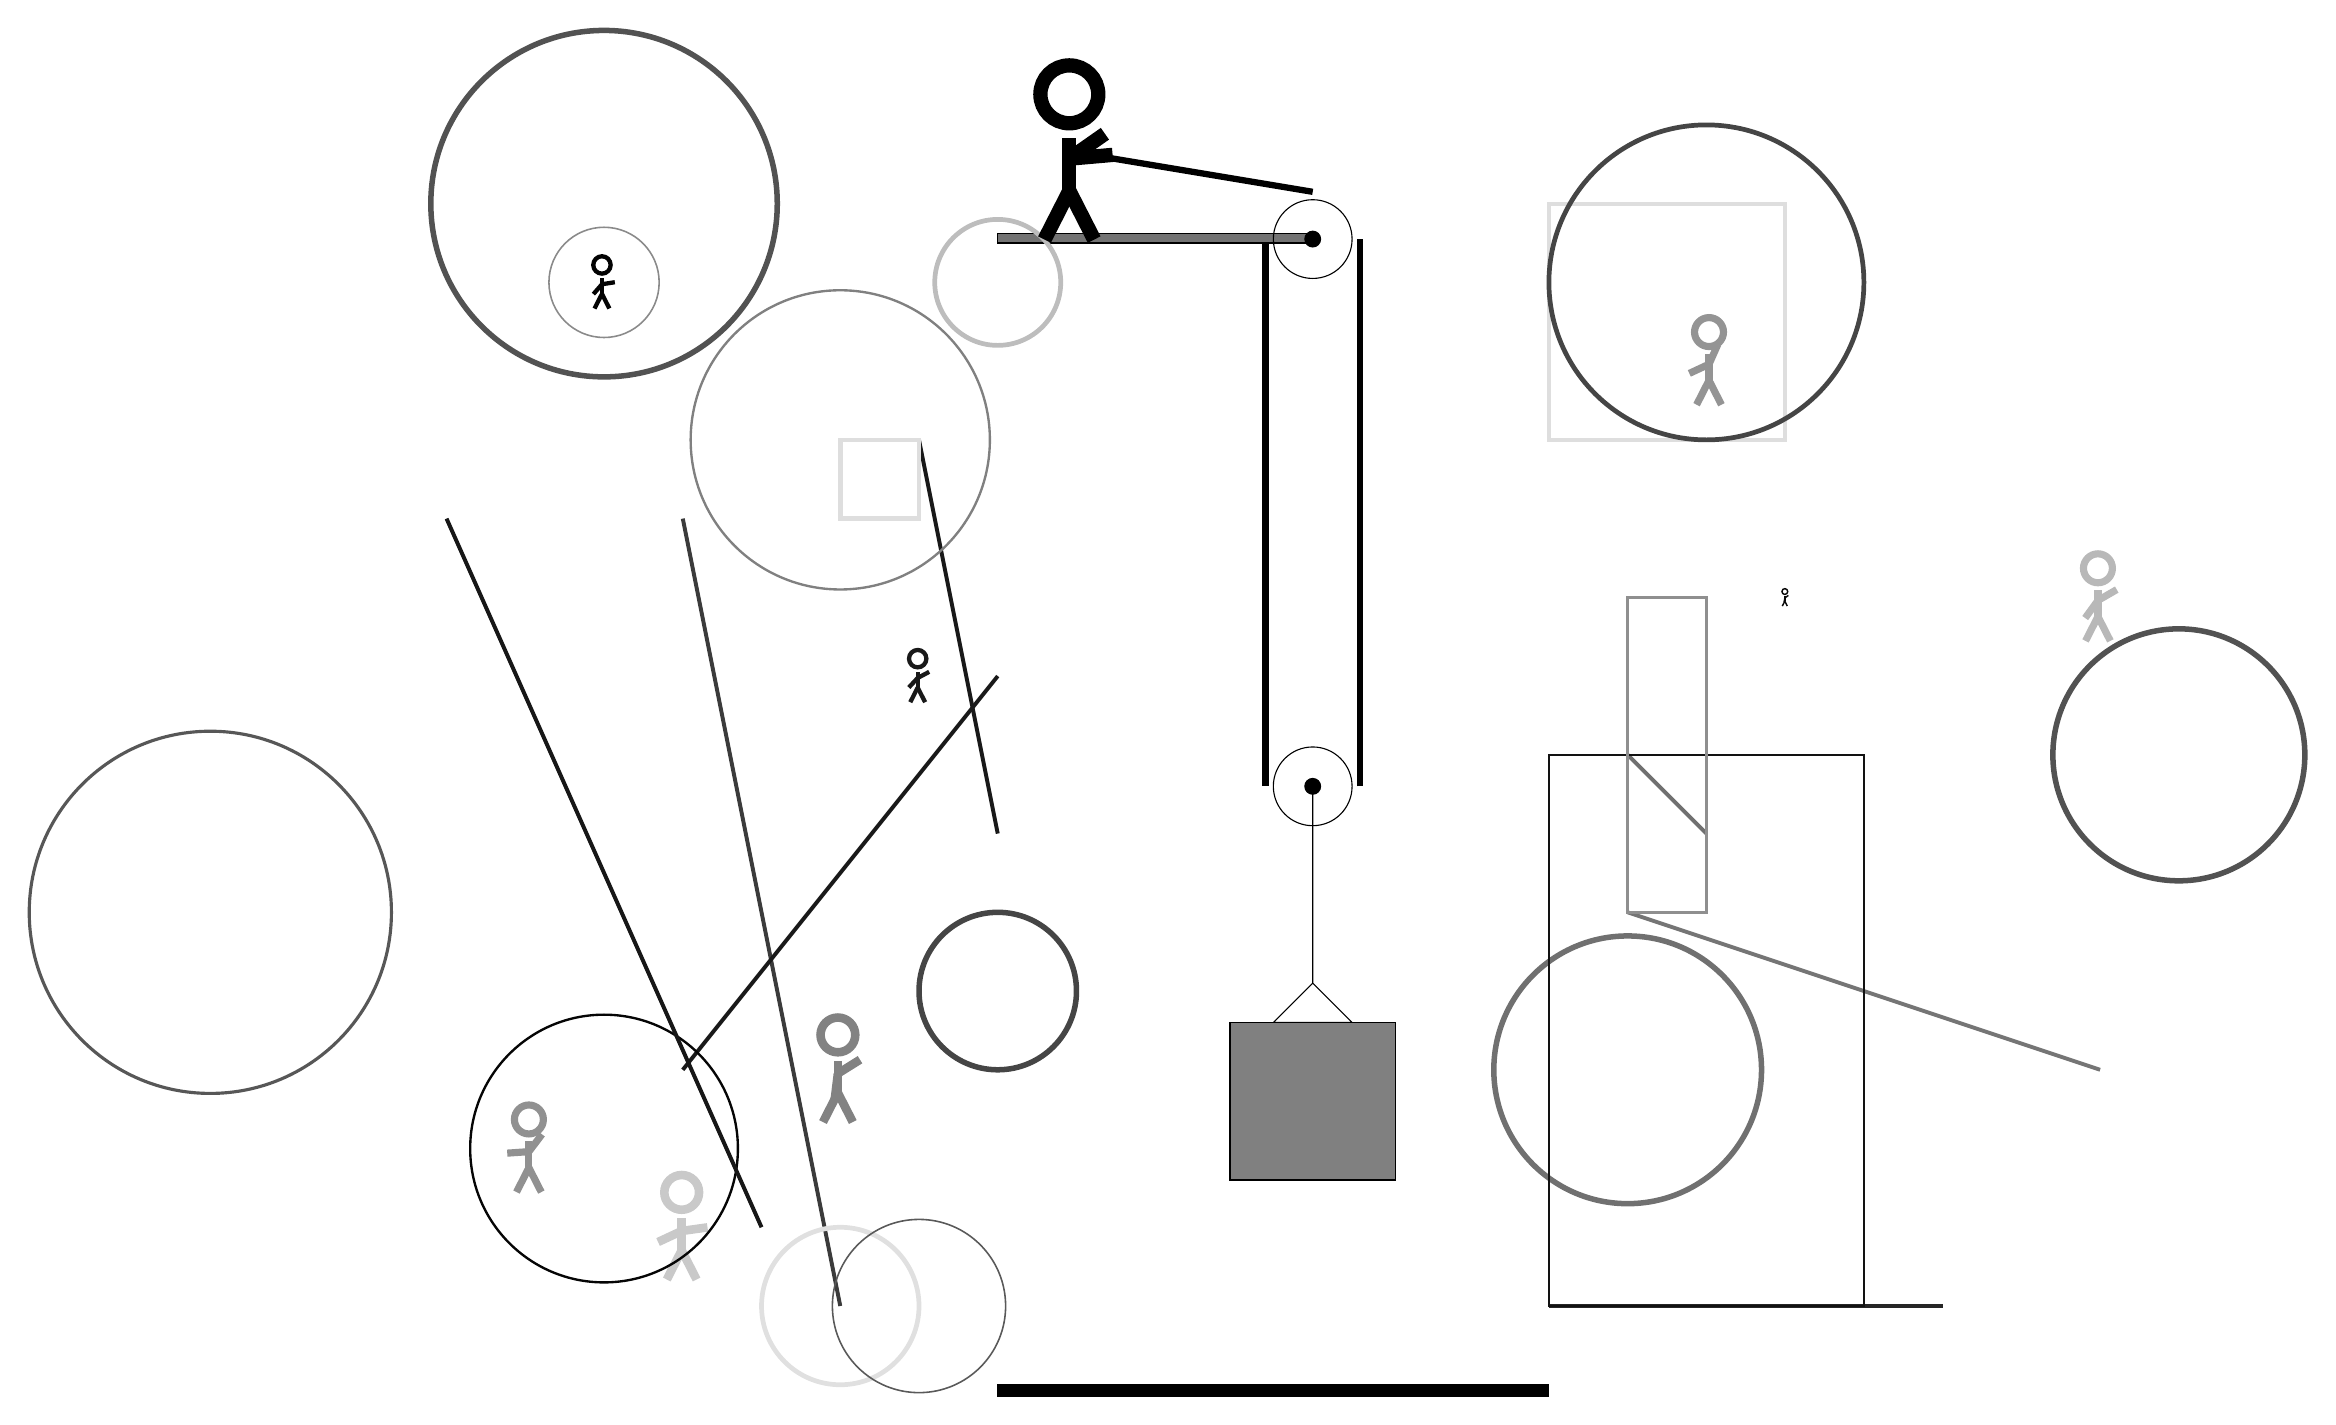
\begin{tikzpicture}
			%%%%% START %%%%%
			
			\draw[fill=black!55] (-2, 11.5) rectangle (2, 11.625);
			
			\draw (2, 4.6) circle (0.5);
			\draw[fill=black] (2, 4.6) circle (0.1);
			
			\draw (2, 11.55) circle (0.5);
			\draw[fill=black] (2, 11.55) circle (0.1);
			
			\draw (2, 4.6) -- (2, 2.1) -- (1.5, 1.6) -- (2.5, 1.6) -- (2, 2.1);
			\draw[fill=black!50] (0.95, 1.6) rectangle (3.05, -0.4);
			
			\draw[line width=0.8mm] (1.4, 11.5) -- (1.4, 4.6);
			\centerarc[line width=0.8mm](2, 4.6)(180:360:0.6);
			\draw[line width=0.8mm](2.6, 4.6) -- (2.6, 11.55);
			\centerarc[line width=0.8mm](2, 11.55)(0:90:0.6);
			\draw[line width=0.8mm](2, 12.15) -- (-1, 12.65);
			
			\node[line width=0.2mm, color=black!43] at (-8, 0) {\Strichmaxerl[5][4][53]};
			
			\draw[line width=0.5mm, color=black!13] (5, 12) rectangle (8, 9);
			\draw [line width=0.7mm, color=black!73](-2, 2) circle (1.0);
			\node[line width=0.7mm, color=black!90] at (-3, 6) {\Strichmaxerl[3][47][28]};
			
			\draw[line width=0.5mm, color=black!77](-6, 8) -- (-4, -2);
			\draw[line width=0.5mm, color=black!90](-6, 1) -- (-2, 6);
			
			\draw [line width=0.7mm, color=black!56](6, 1) circle (1.7);
			\draw [line width=0.6mm, color=black!26](-2, 11) circle (0.8);
			\draw[line width=0.5mm, color=black!85](5, -2) -- (10, -2);
			\node[line width=0.2mm, color=black!42] at (7, 10) {\Strichmaxerl[5][25][66]};
			
			\draw [line width=0.7mm, color=black!68](13, 5) circle (1.6);
			\draw[line width=0.5mm, color=black!90](-3, 9) -- (-2, 4);
			\node[line width=0.7mm, color=black!21] at (-6, -1) {\Strichmaxerl[6][25][8]};
			
			\draw [line width=0.6mm, color=black!12](-4, -2) circle (1.0);
			\draw[line width=0.6mm, color=black!13] (-4, 8) rectangle (-3, 9);
			\draw [line width=0.3mm, color=black!50](-4, 9) circle (1.9);
			
			\draw [line width=0.3mm, color=black!98](-7, 0) circle (1.7);
			\node[line width=0.4mm, color=black!28] at (12, 7) {\Strichmaxerl[5][54][30]};
			\draw[line width=0.5mm, color=black!91](-5, -1) -- (-9, 8);
			
			\draw [line width=0.7mm, color=black!68](-7, 12) circle (2.2);
			\draw [line width=0.2mm, color=black!65](-3, -2) circle (1.1);
			
			\node[line width=0.6mm, color=black!99] at (-7, 11) {\Strichmaxerl[3][49][9]};
			\draw [line width=0.4mm, color=black!66](-12, 3) circle (2.3);
			\draw[line width=0.5mm, color=black!56](7, 4) -- (6, 5);
			\node[line width=0.4mm, color=black!97] at (8, 7) {\Strichmaxerl[1][80][36]};
			
			\draw [line width=0.2mm, color=black!46](-7, 11) circle (0.7);
			\draw [line width=0.6mm, color=black!73](7, 11) circle (2.0);
			\draw[line width=0.5mm, color=black!54](6, 3) -- (12, 1);
			\draw[line width=0.2mm, color=black!93] (5, 5) rectangle (9, -2);
			\draw[line width=0.4mm, color=black!44] (6, 3) rectangle (7, 7);
			\node[line width=0.6mm, color=black!49] at (-4, 1) {\Strichmaxerl[6][83][32]};
			
			
			\node at (-1, 12.65) {\Strichmaxerl[10][-175][35]};
			
			\draw[fill=black] (-2, -3) rectangle (5, -3.15);
			
			%%%%% END %%%%%
		\end{tikzpicture}
	\end{figure}	
\end{document}